\documentclass{article}

\usepackage[letterpaper,top=2cm,bottom=2cm,left=2cm,right=2cm,marginparwidth=1.75cm]{geometry}

\usepackage{amsmath}
\usepackage{graphicx}
\usepackage{titlesec}
\usepackage{lipsum}
\usepackage{mwe}
\usepackage[parfill]{parskip}
\usepackage[colorlinks=true, allcolors=blue]{hyperref}

\pdfpagewidth=8.5in
\pdfpageheight=11in


\def\tricolfig#1{\includegraphics[width=2.2in]{#1}}
\def\triplecolfig#1{\includegraphics[width=0.32\textwidth]{#1}}
\def\smallcolfig#1{\includegraphics[width=2.0in]{#1}}
\def\smallercolfig#1{\includegraphics[width=0.75\columnwidth]{#1}}
\def\mediumcolfig#1{\includegraphics[width=0.9\columnwidth]{#1}}
\def\colfig#1{\includegraphics[width=\columnwidth]{#1}}
\def\pagefig#1{\includegraphics[width=0.75\textwidth]{#1}}
\def\suspcolfig#1{\includegraphics[width=2.0in]{#1}}
\def\perfcolfig#1{\smallercolfig{#1}}



\def\crcd{compiler-runtime co-design}
\def\ALL{allocation}
\def\DALL{deallocation}
\def\ALLS{allocations}
\def\DALLS{deallocations}
\def\DWS{dynamic memory working set size}
\def\SIZE{allocation size}
\def\SIZES{allocation sizes}



\title{Compiler and Runtime Support for Functions-as-a-Service (FaaS)}
\date{}
\author{Souradip Ghosh, 15-849, Fall 2021}

\begin{document}
\maketitle

\section{Abstract}
Functions-as-a-Service (FaaS) are rapidly growing in popularity and 
complexity among cloud service provides as users look to take 
advantage of cloud resources on-demand and focus on computation
at a finer grain. FaaS instances are characteristically short-lived
and often dominated by communication and cold-start overheads compared
to typical monolithic applications. At the same time, FaaS instances
are requiring more resources, especially memory, to operate. Although
many works have approached these issues with scheduling optimizations,
hardware accelerators, and other techniques, very few have examined
\textit{compiler} support and \textit{\crcd} for FaaS. This paper presents 
a \crcd\ consisting of static analyses, profiling, and a custom memory 
allocator controlled by the compiler and runtime to better understand 
and optimize \textit{dynamic memory usage} for small FaaS workloads.

\section{Introduction/Background}

\section{Design}
The design of the system consists of three major components : 1) a \textit{profiler},
2) \textit{static analyses} in the compiler, and 3) a \textit{custom memory allocator}
that is \textit{designed and optimized with FaaS characteristics in mind}. The first and third components consist 
of compiler instrumentation coupled with an integrated runtime. All analyses and 
transformations operate on the \textit{intermediate representation} (IR) of the compiler, 
where standard compiler optimizations are performed. These components are described in 
the following subsections in detail. 

\begin{figure}
    \centerline{\pagefig{figs/sys.pdf}}
    \caption{System overview and compilation pipeline. }  
	\label{fig:sys}
\end{figure}

An overview of the system and compilation pipeline is show in Figure~\ref{fig:sys}. The 
first pass over an example workload (\texttt{app.c}) consists of static analyses and 
profiling. The second pass over \texttt{app.c} instruments the program with the custom
allocator using the results from the static analyses (and optionally the profiler). This 
custom allocator replaces standard dynamic \ALLS\ and \DALLS\ in \texttt{app.c}, and it is
the \textit{crux} of optimization for dynamic memory usage in FaaS workloads. The
outputs from this compilation pipeline include an instrumented application (\texttt{app.exe})
and statistics about \DWS\ (total size for all dynamic \ALLS).

\subsection{Profiler}
The profiler has the goal of understanding information about dynamic memory \ALLS\ and 
\DALLS\ during execution (for instance, the number of \ALLS\, \DWS\, common \ALL 
sizes, etc.) as well as standard information about the "hotness" of functions and
loops at runtime. Using this data, the profiler can inform the compiler during 
instrumentation in the second pass over the application (see \ref{ca}). It can also 
inform the user with a better estimate of memory usage for a future FaaS instance or 
function invocation.

The profiler tracks all \ALLS and \DALLS of some workload, $W$, at runtime. This is 
accomplished by using the compiler to instrument all explicit dynamic memory \ALL\ and \DALL\ function 
calls in the IR for $W$ with \textit{callback} functions to a profiler runtime.
Two callbacks, \texttt{TrackAllocation(ptr, size)} and \texttt{TrackDeallocation(ptr)}, are 
sufficient to achieve all tracking. \texttt{TrackAllocation} takes a pointer to an allocation (\texttt{ptr}) and 
the size of the allocation (\texttt{size}) as inputs and records the pair in a table in the 
profiler's runtime. \texttt{TrackDeallocation} simply takes a pointer to an allocation (\texttt{ptr}) as
input and removes the entry from the profiler runtime's table. An example of this 
instrumentation is shown in Figure~\ref{fig:pins}.

\begin{figure}
    \centering
    \begin{minipage}{0.45\textwidth}
        \centering
        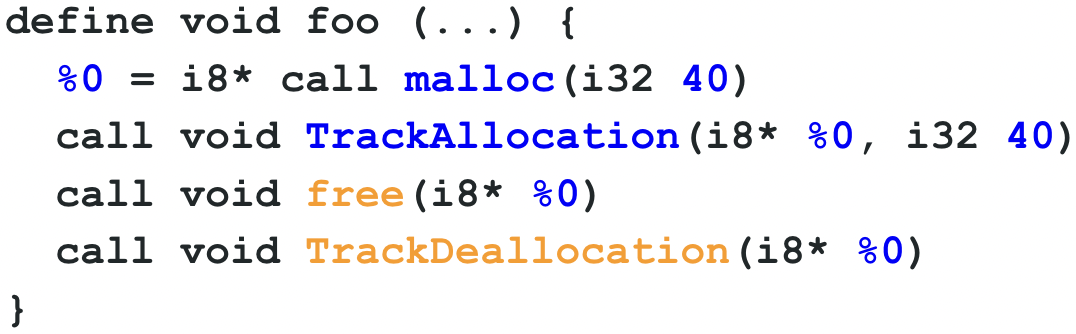
\includegraphics[width=0.9\textwidth]{figs/pins.png} 
        \caption{Example compiler instrumentation for profiler callbacks in the 
        context of simplified LLVM IR and \textit{libc} \texttt{malloc}
        and \texttt{free}}  
	    \label{fig:pins}
    \end{minipage}\hfill
\end{figure}

While $W$ runs, the profiler tracks each change to the \DWS\ over its entire execution 
whenever a callback is invoked. Using this information, the profiler calculates maximum 
and average \DWS\ for $W$ and outputs the data to the user and to the compiler for future 
use. All profiler information can be optionally used by the custom allocator component of
the \crcd\ (see \ref{ca}).

\subsection{Static Analyses}
The system also supports static analyses of \ALLS\ and \DALLS\ in the IR for workload $W$. 
In particular, the compiler analyzes 1) \ALL\ sizes for all \ALLS\, 2) loops to unroll 
and functions to inline so that 1) is more feasible to analyze, and 3) uses of \ALL\ and 
\DALLS . All analyses informs the compiler about analyzable static allocations. 

The first analysis is especially important to identify \ALL\ and \DALL\ candidates that
can be replaced with the custom allocator. At a high level, the "easier it is to deduce"
the allocation \textit{size} for each \ALL\, the easier it is to replace the \ALL\ with one
of the methods from the custom alloactor (see \ref{ca} for details).

An "easy-to-deduce" or \textit{statically analyzable} \SIZE\ is one that is 
simply a constant integer. All other \SIZES\ are \textit{analyzable with
assistance}, where the size can apparently be deduced during runtime. These 
categories are mutually exclusive. The compiler records all statically analyzable 
\SIZES .

Some \SIZES\ that are analyzable with assistance are worth recording, however. In
particular, if an \SIZE\ is dependent on function arguments, the function (and
its parent functions) can be continually inlined until the size is statically
analyzable. Consequently, the compiler marks functions that are candidates for
aggressive inlining (compared to a standard inliner in \texttt{-O3}). At an
extreme, aggressive inlining can reach a point where it may be beneficial to
inline the entry-point function of $W$. This is especially common in small 
FaaS workloads where \ALLS\ towards the beginning of the workload havew \SIZES\
dependent on the inputs. Obviously, inlining the entry-point function is not 
possible, but we can borrow concepts from JIT compilation or binary translation
to possibly embed the inputs into the binary itself. This process can occur
right before the $W$ is invoked in the FaaS instance. A subset of this system's compiler
can analyze and transform $W$ as necessary. This solution is theoretical and 
not applied in this work.

Additionally, \SIZES\ that exists in a loop and are dependent on loop-invariant
values are also recorded. Here, the loop itself can be aggressively unrolled and
the \ALLS\ can be merged or replaced with one of the methods from the custom 
allocator. It is also important that the size is dependent on a loop-invariant 
value, or else the compiler cannot affirmatively analyze multiples of the size or
determine an appropriate unroll factor (unrolling too much without knowledge of
the \SIZE\ may be sub-optimal).

Finally, the compiler analyzes the uses of \ALLS , especially if they are used
in explicit \texttt{store} operations in the IR. An \ALL\ pointer that is stored
to an arbitrary memory location is an \textit{escape}, and it is very difficult
to analyze its value, lifetime, and size once it leaves the scope of its parent
function. Additionally, it is hard to manage \DALLS\ if pointer origins
cannot be deduced, which can be common with escaped \ALL\ pointers. All escapes
are recorded. All \ALLS\ and \DALLS\ that cannot be statically analyzed using
memory alias analysis (i.e "must alias" conditions) or def-use chains are flagged.

\subsection{Custom Allocator} \label{ca}

\section{Implementation}

\section{Evaluation}

\section{Future Work}

\section{Conclusion}

\bibliographystyle{plain}
\bibliography{sample}

\end{document}
